\documentclass{article}

\usepackage{amsmath}
\usepackage{hyperref}
\usepackage{natbib}
\usepackage{algorithm}
\usepackage{algpseudocode}
\usepackage{graphicx}
\usepackage{xcolor}
\usepackage{tikz}
\usetikzlibrary{arrows.meta, calc}
% \usepackage{showframe}

\hypersetup{
    colorlinks,
    linkcolor={red!50!black},
    citecolor={blue!50!black},
    urlcolor={blue!80!black}
}

\graphicspath{ {.} }

\begin{document}
\noindent\makebox[\textwidth][c]{\Large\bfseries Neural Networks}

\tableofcontents

\section{Loss Functions}

Also known as an {\em objective function}, {\em criterion}, {\em cost function}, or {\em error function}.

\subsection{Classification}

\subsubsection{Log/Cross Entropy loss}

In binary classification (where $y \in \{ 0, 1 \}$),

\begin{align}
    L_i &= -(y_i \log(p_i) + (1 - y_i) \log(1 - p_i)) \\
    L &= \frac{1}{N} \sum_{i=1}^{N} L_i
\end{align}

\noindent
Note that only the correct class contributes to the value of $L_i$ (the other term is zero). To have no loss, we need $p = y$. As $0 < p_i < 1$, the value of both $\log$'s are negative, hence the outer negation to create a positive loss.

We can generalize this to classification problems with $M > 2$ possible classes by writing,

\begin{equation}
    L_i = - \sum_{c = 1}^{M} y_{i, c} \log(p_{i, c})
\end{equation}

\noindent
where $y_{i, c} = 1$ if the class $c$ is the correct class and $0$ otherwise and $p_{i, c}$ is the probability we assigned to that class.

\subsubsection{Precision, Recall, and F-measure}

Assume we have an event (True, False) and a model the predicts (Positive, Negative). Then, define precision as ``the fraction of positives of the model that were true''.

\begin{equation}
    {\rm Precision} = \frac{\rm True\ positives}{\rm All\ positives}
\end{equation}

\noindent
and recall as ``the fraction of true events that were positives''.

\begin{equation}
    {\rm Recall} = \frac{\rm True\ positives}{\rm All\ true}
\end{equation}

When a high precision classifier calls something positive, it is usually true (but unless it is high recall, it might call many true events false too).
When a high recall gets a true event, it will usually call it positive (but unless it is precise it will also call many other things positive).
A related concept useful for showing this data to people is the confusion matrix. This is a $2 \times 2$ matrix with columns of the event (True, False) and rows with the prediction (Positive, Negative) and the counts in each cell.

\begin{figure}[h!]
    \centering
    \href{https://en.wikipedia.org/wiki/Precision_and_recall}{
        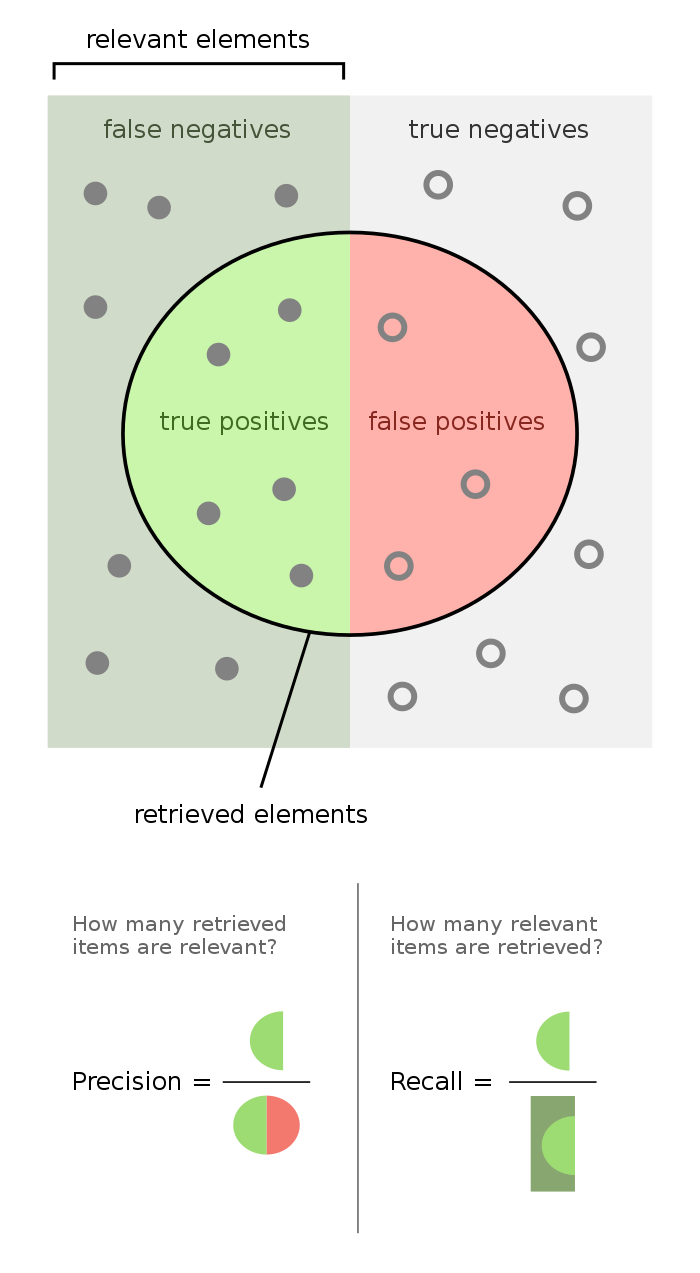
\includegraphics[width=0.6\textwidth]{./figures/PrecisionRecall.png}
    }
\end{figure}

While performance and recall are useful, we generally want to summarize performance with a single number. This can be done with the ``F-measure'' (or F-score).

\begin{equation}
    F = 2 \frac{p \cdot r}{p + r}
\end{equation}

To show why we might want to use this, consider a classifier for a rare event (say a medical test where we expect only 1\% of the population to have the disease).
A naive classifier could easily achieve 99\% accuracy just by returned negative for everyone, and so the naive ``accuracy'' classifier would be bad.
However, that naive classifier would have recall of $0$ and therefore a terrible F-score.

We often need to trade recall for precision. In the medical example above, as we start to claim positives in some situations our recall will improve (as we identify some true positives) but our precision will decrease (as we identify as true some negatives). We can think of this as changing the threshold on a model that outputs something that looks like a probability.

If we plot a figure with axes of (precision, recall), models with extremely low thresholds will sit roughly at (0, 1) or (terrible precision because there are so many positives, great recall because everything is positive). Models with high thresholds will sit at (1, 0) or (great precision because we only claim a positive if we are really sure, terrible recall because of that high threshold).
A good model will also have a point near (1, 1) rather than trending down the $r = p$ line.
We can show this in \autoref{fig:ROC} which shows something slightly different (slightly different axes), but the same idea.

\begin{figure}[h!]
    \centering
    \href{https://towardsdatascience.com/handling-imbalanced-datasets-in-machine-learning-7a0e84220f28}{
        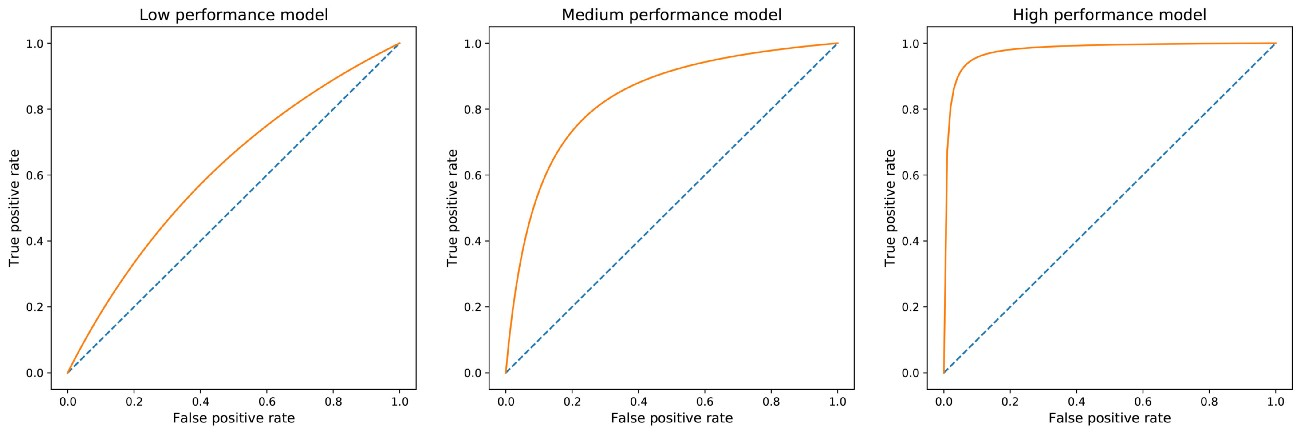
\includegraphics[width=0.97\textwidth]{./figures/ROC.jpeg}
    }
    \label{fig:ROC}
\end{figure}


\subsection{Regression}

\subsubsection{Mean Squared Error (MSE)}
\section{Activation Functions}

% Can't put in table
% $$
% \begin{cases} 
%     0 &\quad x < 0 \\
%     x &\quad x > 0 
% \end{cases} 
% $$

\begin{center}
\begin{tabular}{ l l l l l }
 \hline
 Name & Function & Range & Differentiable? & Zero centered \\
 \hline
Rectified Linear Unit (ReLU)    & 
x
                                                                    & $ [0, \infty) $   & Everywhere except 0   & No \\
 Sigmoid                        & $\sigma(x) = \frac{1}{1+e^{-x}}$  & $ (0, 1) $        & Yes                   & No \\
 Tanh                           & F                                 & $ (-1, 1) $       & Yes                   & Yes \\
 \hline
\end{tabular}
\end{center}



\subsection{ReLU (Rectified Linear Unit)}

The ReLU activation function is simply,

\begin{equation}
    \max(0, x)
\end{equation}

\noindent
While simple, this activation has many advantages. ``Because rectified linear units are nearly linear, they preserve many of the properties that make linear models easy to optimize with gradient-based methods'' \citet[pg.~169]{Goodfellow2016}.
However, also note that ReLU can also kill neurons (as there is no gradient when $x < 0$.

Use this as your activation function unless you have a good reason not to.

\subsection{Sigmoid (logistic)}

The sigmoid function is defined as,

$$
\sigma(x) = \frac{1}{1 + e^{-x}}
$$

\noindent
with key values of,
\begin{align}
    \sigma(0) = 0.5 \\
    \lim_{x \to \infty} \sigma(x) = 1 \\
    \lim_{x \to -\infty} \sigma(x) = -0
\end{align}

\noindent
The downside of sigmoid activations is that as $x$ gets far from $0$, the gradient is essentially flat. This stops backprop.

\subsection{Hyperbolic Tangent (Tanh)}

Basically the same as sigmoid except the key values are,

\begin{align}
    \sigma(0) = 0 \\
    \lim_{x \to \infty} \sigma(x) = 1 \\
    \lim_{x \to -\infty} \sigma(x) = -1
\end{align}

\subsection{Softmax}

Softmax is often used in multiclass classification problems. It takes a vector of real numbers and normalizes it into a probability distribution ($0 \leq p_i \leq 1$, $\sum_{i} p_i = 1$). If we call the input vector $z$, the output vector $\sigma(z)$, both of which have length $k$, it is defined as:

$$
\sigma(z)_i = \frac{ e^{z_i} }{ \sum_{j=1}^{k} e^{z_j} }
$$

This makes sense if we interpret the output layer before the activation function as a log likelihood. Softmax converts log likelihood to a probability.


\section{Backpropagation}

Backpropagation (or just backprop) is a method for computing the gradient. Specifically we are interested in $\nabla_{x} f(x, y)$, where $f$ is an arbitrary function, $y$ are inputs to the function whose derivatives we are not interested in, and $x$ are variables whose derivatives we want.
For machine learning, those $x$ are the parameters (weights and biases) of the neurons.

It is maybe nicer to think about this not as finding the gradient (a vector in high dimensional space pointing downhill) but rather as finding the sensitivity of the cost to each parameter (a bunch of partial derivatives).
It amounts to the same thing, but one is easier to visualize that the other.

\subsection{A single neuron (Final Layer)}

Let's first look at the last layer ($L$) of a network that has a single neuron, and a single incoming activation (the previous layer also had a single neuron). We assume a MSE loss function and a sigmoid activation function.

\begin{align}
    z^{(L)} &= w^{(L)} a^{(L - 1)} + b^{(L)} \\
    a^{(L)} &= \sigma(z^{(L)}) \\
    C &= (a^{(L)} - y)^2
\end{align}

\noindent
We want to know how the weight $w^{(L)}$ and bias $b^{(L)}$ on this layer effect the cost $C$.
$$
\frac{\partial C}{\partial w^{(L)}} \text{  and  }
\frac{\partial C}{\partial b^{(L)}}
$$
As we have represented the process as a nested sequence of functions,
$$
C = \text{cost}(\text{activation}(\text{affine}(a^{(L - 1)})))
$$
this derivative can be computed using the chain rule\footnote{
Given $h(x) = f(g(x))$ the chain rule tells us that $h'(x) = f'(g(x)) \cdot g'(x)$ or ``the derivative of the outer evaluated at the inner multiplied by the derivative of the inner''. But, if we assign the output of the inner function to an intermediate variable, $y = g(x)$ and the output for the combination to $z = f(g(x)) = h(x)$, we can rewrite this as $h'(x) = f'(y) \cdot g'(x)$ or more suggestively $ \frac{dz}{dx} = \frac{dz}{dy} \frac{dy}{dx} $.
}.


\begin{equation}
    \frac{\partial C}{\partial w^{(L)}} = \frac{\partial C}{\partial a^{(L)}} \frac{\partial a^{(L)}}{\partial z^{(L)}} \frac{\partial z^{(L)}}{\partial w^{(L)}}
    \label{eq:finalLayerChain}
\end{equation}

\noindent
Evaluating all these derivatives gives us,

\begin{align}
    \frac{\partial C}{\partial w^{(L)}} &= 2(a^{(L)} - y) \cdot \frac{e^{-z^{(L)}}}{(1 - e^{-z^{(L)}})^2} \cdot a^{(L - 1)} \\
    \frac{\partial C}{\partial b^{(L)}} &= 2(a^{(L)} - y) \cdot \frac{e^{-z^{(L)}}}{(1 - e^{-z^{(L)}})^2}
\end{align}

What does this tell us? Let's assume $a^{(L)} < y$. Then the first term $2(a^{(L)} - y)$ is negative. The second term is always positive as the sigmoid function increases monotonically. Thus $\frac{\partial C}{\partial b^{(L)}} < 0$ which means that increasing the bias decreases the cost. This makes sense as increasing $b^{(L)}$ increases $z^{(L)}$ and $a^{(L)}$. Conversely if $a^{(L)} > y$ increasing the bias will increase the cost.
The weight follows a similar argument, though the signs will switch if $a^{(L - 1)} < 0$.

Which factor is more efficient at impacting the cost? This depends entirely on the incoming activation. If $|a^{(L - 1)}| > 1$ the cost responds more to the weight than the bias.


\subsection{A Single Neuron (Hidden Layer)}

We've seen how to compute the derivative of the cost w.r.t. the bias and weight of the final layer. How do we do the same for previous layers?

We can extend \autoref{eq:finalLayerChain} to the previous layer,

\begin{equation}
    \frac{\partial C}{\partial w^{(L - 1)}} =
        \frac{\partial C}{\partial a^{(L)}}
        \frac{\partial a^{(L)}}{\partial z^{(L)}}
        \frac{\partial z^{(L)}}{\partial a^{(L - 1)}}
        \frac{\partial a^{(L - 1)}}{\partial z^{(L - 1)}}
        \frac{\partial z^{(L - 1)}}{\partial w^{(L - 1)}}
    \label{}
\end{equation}

\noindent
where the only new ingredient is,

\begin{equation}
    \frac{\partial z^{(L)}}{\partial a^{(L - 1)}} = w^{(L)}
\end{equation}

\noindent
This can be understood nicely with a graph,

\begin{tikzpicture}[scale = 10]
\begin{scope}[every node/.style={}]

    \node (C) at (1, 0.5) {$C$};
    % layer
    \node (A_L) at (0.75, 0.5) {$a^{(L)}$};
    \node (y) at (0.75, 0.3) {$y$};
    % Layer
    \node (Z_L) at (0.5, 0.5) {$z^{(L)}$};
    % Layer
    \node (A_L1) at (0.25, 0.5) {$a^{(L - 1)}$};
    \node (W_L) at (0.25, 0.3) {$w^{(L)}$};
    \node (B_L) at (0.25, 0.7) {$b^{(L)}$};
    % Layer
    \node (Z_L1) at (0, 0.5) {$z^{(L - 1)}$};
\end{scope}

\begin{scope}[
    every edge/.style={draw=blue,thick}
]
    \path [->] (A_L) edge (C);
    \path [->] (y) edge (C);
    % Layer
    \path [->] (Z_L) edge node[above] {$\sigma$} (A_L);
    % Layer
    \path [->] (W_L) edge (Z_L);
    \path [->] (B_L) edge (Z_L);
    \path [->] (A_L1) edge (Z_L);
    % Layer
    \path [->] (Z_L1) edge node[above] {$\sigma$} (A_L1);
\end{scope}
\end{tikzpicture}

\noindent
Backpropagation walks backwards (from $C$) along this graph, keeping track of the derivative as it goes. So,

\begin{align}
    \textcolor{red}{\frac{\partial a^{(L)}}{\partial C}} &= 2 (a^{(L)} - y) \\
    \textcolor{blue}{\frac{\partial z^{(L)}}{\partial C}} &= \sigma '(z^{(L)}) \cdot \textcolor{red}{\frac{\partial a^{(L)}}{\partial C}} \\
    % Layer
    \frac{\partial b^{(L)}}{\partial C} &= \textcolor{blue}{\frac{\partial z^{(L)}}{\partial C}} \\
    \textcolor{purple}{\frac{\partial a^{(L - 1)}}{\partial C}} &= w^{(L)} \cdot \textcolor{blue}{\frac{\partial z^{(L)}}{\partial C}} \\
    \frac{\partial w^{(L)}}{\partial C} &= a^{(L - 1)} \cdot \textcolor{blue}{\frac{\partial z^{(L)}}{\partial C}} \\
    % Layer
   \textcolor{orange}{\frac{\partial z^{(L - 1)}}{\partial C}} &=  \sigma '(z^{(L-1)}) \cdot \textcolor{purple}{\frac{\partial a^{(L - 1)}}{\partial C}} &
\end{align}


\section{Data Inputs}


\subsection{Categorical Data in Neural Nets}

While some ML algos can handle categorical data easily (e.g. random forests), it is not immediately obvious how neural nets can deal with them.

One bad idea would be to simply assign an integer to each category. However, while this will get things to work, this feature will likely be nothing but misleading.

One hot encoding is a good thing to do (as long as the feature does not have too high cardinality). Imagine we have ["red", "green", "blue"] as a car color in a model for number of accidents. We could map red to [1, 0, 0], green to [0, 1, 0] and blue to [0, 0, 1].
For high cardinality data, OHE is not possible (as the input vector would be large).

Sometimes, if there is an ordering, we might be able to do better than one hot. For example, if the classes relate to amount of education, [High school, Undergrad, Masters, PhD] it may be reasonable to represent those as integers representing the number of years of schooling (or something similar).

\subsubsection{Embeddings}

These seem quite important.

An embedding is a low-dimensional, learned, continuous, vector representation of discrete variables.

\subsection{High Cardinality Categorical Inputs}


\section{Regularization}

Regularization is any process or strategy that aims to reduce the error on the test set (generalization error), but not its training error.
There are many ways to do this.

One way to think about regularization (which appeals to me) comes from \citet{Srivastava2014}. They say,
``With unlimited computation, the best way to “regularize” a fixed-sized model is to
average the predictions of all possible settings of the parameters, weighting each setting by its posterior probability given the training data.''
This naturally leads to ensemble methods, but these are computationally expensive.


\subsection{Parameter Norm Penalties}

Rather than minimize the loss function $L(\theta, X, y)$, instead minimized,

$$
L'(\theta, X, y) = L(\theta, X, y) + \alpha \Sigma(\theta)
$$

\noindent
where $0 < \alpha < \infty$ (and $\alpha = 0$ corresponds to no regularization).
The choice of $\Sigma$ is relatively free.
Two popular options are the $L^2$ and $L^1$ norms.

\begin{align}
    \text{L2:} || \theta ||_2 =& \sqrt{x_1^2 + \cdots + x_n^2} \\
    \text{L1:} || \theta ||_1 =& | x_1 | + \cdots + | x_n |
\end{align}

These have different effects. The L1 norm promotes sparsity.

Note that the choice of $\alpha$ is a hyperparameter that requires many training runs (and then a check against a validation set) to optimize.

\subsection{Dataset Augmentation}

One source of generalization error is that we train on only a subset of possible examples. If we can train on a wider variety of possible inputs, we will have a more general network.

Exactly what forms of augmentation are available depend on the problem. However some suggestions are,

\begin{itemize}
    \item Addition of noise (e.g. Gaussian noise on top of an image)
    \item Rotation/transformation/scaling of the image (though not when that would change the meaning (b d) or result in unlikely data (upside down photos))
\end{itemize}


\subsection{Early Stopping}

While we might usually train until the error on the training set plateaus, this can lead to overfitting. With early stopping, we train until we get the best performance on the validation set.

We can think of this as a hyperparameter (amount of training) selection algorithm (which is the point of the validation set!).

\subsection{Bagging/Ensemble Methods}

{\bf B}ootstrap {\bf agg}regat{\bf ing} reduces generalization error by training several models (which will hopefully have independent errors) and using the average of their prediction for inference. These are known as ensemble methods because we have use an ensemble of models!

Some math in \citet[pg. 249]{Goodfellow2016} explaining that the error goes as $1/k$ with $k$ totally uncorrelated models.

\subsection{Dropout}

This comes from \citet{Srivastava2014}.

We can think of a neural net as a graph with $2^n$ possible subgraphs (or thinned networks).
Note that in small networks, a large fraction of thinned networks will have no valid path from input to output, but that this fraction is negligible in larger ones.
With dropout, each training iteration uses a different thinned network where each node is present with some probability $p$ (dead nodes output 0).
The weights of each node is the same in all thinned networks.
The hope is that the weights will converge to the geometric mean of the posterior distribution. This is likely the best we can do without training an ensemble that allows us to sample from the full posterior.
At test time, the unthinned network is used, with the weights scaled by $p$ (to account for the unthinning!)

Typical values for $p$ are,

\begin{align}
    p_{\rm hidden} &\sim 0.5 \\
    p_{\rm input} &\sim 0.8
\end{align}


\section{Optimization}

\subsection{The Gradient}

Before looking specifically at optimization methods, we should remind ourselves what the gradient is. Mathematically the gradient of a scalar valued function $f$ of several variables has a value at point $x$ of,

\begin{equation}
    \nabla f(x) = \begin{bmatrix}
        \frac{df}{dx_{1}} \\
        \vdots \\
        \frac{df}{dx_{n}} \\
    \end{bmatrix}
\end{equation}

\noindent
This can be thought of as a generalization of the derivative (which gives the rate of increase) to multivariate functions. The gradient gives the direction of greatest increase as well as the rate in that direction.

If the gradient points up the slope, $-\nabla f(x)$ points in the direction of greatest decrease in the function. If the function is linear, we can find the roots (where $f(x) = 0$) in a single step using Newton's method,

\begin{equation}
    x_1 = x_0 - \nabla f(x_0) \frac{f(x_0)}{\nabla f(x_0)  \cdot \nabla f(x_0)}
\end{equation}

\noindent
Practically, the function is not linear and may not have any roots (in ML, these might only exist where the loss is 0). What we are interested in finding is the location where $f(x)$ is minimized, i.e. where the {\em gradient\/} is 0.

\subsection{Gradient Descent}

Now that we understand what the gradient is, and why we can't use it to immediately jump to the perfect parameter values (there might not be any roots, function is certainly non linear, we can't estimate the gradient perfectly) we can think about how we can use it.

The obvious thing to do is just to move in the opposite direction to the gradient. How far to step though is unclear. We solve this by adding a hyperparameter $\epsilon$ (known as the learning rate) which can be tuned for the problem. This needs to be small enough so that the gradient doesn't change too much along our step but large enough to not require a large number of estimates of the gradient.

\begin{algorithm}
\begin{algorithmic}
    \Require{} Learning rate $\epsilon$
    \Require{} initial state $\theta$
    \While{---}
        \State{} Make an estimate (somehow) of the gradient ($\hat{g}$)
        \State{} Update $\theta = \theta - \epsilon \hat{g}$
    \EndWhile{}
\end{algorithmic}
\end{algorithm}

\subsection{Momentum Gradient Descent}

In the standard gradient descent, each step is independent from the others and depends only on the gradient we estimated at that point. This might sound reasonable (why should previous estimates of the gradient at other points have a say on the current step?) but when the learning rate is small previous gradients {\em are\/} relevant. In fact, if the gradient estimates we get are noisy (from e.g. small minibatch sizes) estimates of the gradient using multiple minibatches from nearby locations can dramatically reduce the number of optimization steps required.

The physical analogy often drawn here is of a ball rolling around a 2d surface. Its velocity is not set directly by the gradient. Rather, the gradient acts as an acceleration, {\em modifying\/} the velocity. This analogy also explains the name of this method as velocity $\propto$ momentum.

\begin{algorithm}
\begin{algorithmic}
    \Require{} Learning rate $\epsilon$, momentum parameter $0 < \alpha < 1$
    \Require{} initial state $\theta$, initial velocity $v \gets 0$
    \While{---}
        \State{} Make an estimate (somehow) of the gradient ($\hat{g}$)
        \State{} Update the velocity $v = \alpha v - \epsilon \hat{g}$
        \State{} Update $\theta = \theta + v$
    \EndWhile()
\end{algorithmic}
\end{algorithm}

Notice that: $\alpha = 0$ is equivalent to the momentum free gradient descent. On the first step, where there is no velocity, the step will also be the same as momentum free gradient descent. The impact of the velocity gained in previous steps decays exponentially as they accumulate factors of $\alpha$ (this can be thought of as drag in the physical analogy. Without this, the particle would not come to rest near a minimum).

What impact does this have on the step size? In the momentum free gradient descent, the largest step is $s = \epsilon g$. With momentum, successive gradients in the same direction result in,

\begin{equation}
    v = s + \alpha s + \alpha^2 s + \cdots + \alpha^n s = s \sum_{n=0}^{\infty} \alpha^n = \frac{s}{1 - \alpha}
\end{equation}

If the steps are in opposite, or near to opposite, directions (e.g. when descending down a narrow valley, we might jump from cliff to cliff),

\begin{equation}
    v = s - \alpha s + \alpha^2 s - \cdots{} + \alpha^n s = s \sum_{n=0}^{\infty} (-\alpha)^n = \frac{s}{1 + \alpha}
\end{equation}

\noindent
Thus momentum allows quicker convergence both by improving the estimate of the gradient, and by increasing the step size when successive gradients are in the same direction (e.g. by a factor of 10 if $\alpha = 0.9$). When the gradient is in opposite directions, the step size is reduced but hopefully in a better direction.


\section{Bias Variance Tradeoff}



\section{Autoencoders}

\bibliographystyle{plainnat}
\bibliography{/home/christopher/research/papers/all}
\end{document}
